\documentclass[a4paper, 10pt, conference]{IEEEtran}      % For A4 Paper
%The Class IEEECONF will be installed by MiKTeX and Texmaker automatically
% All the required Packages will be automatically installed if you have MiKTeX and Texmaker 
\usepackage{algorithm,algpseudocode}

\usepackage{amsmath}
\usepackage{amssymb} 
\usepackage{graphics}
\usepackage{epsfig}
\usepackage{mathptmx}
\usepackage{array}
\usepackage{tabu}
\usepackage{hyperref}
\graphicspath{ {images/} }
% If You use Texmaker it will automatically download missing packages

\title{\LARGE \bf MPI:Game of Life}
% Enter your Title here
% If the title is too long use line breaker (\\) to break into two
% If you do not use line breaker manually, it will be broken automatically by LATEX  

\author{Chirag Majithia}

\begin{document}
	
	
	\maketitle
	\thispagestyle{empty}
	\pagestyle{empty}
	
	
	
	\begin{abstract}
		The aim of the project is to get familiarized to Message Passing Interface (MPI), used in parallel computing. The project uses Open MPI implementation of the MPI standards for solving "Conway's Game of Life" problem.
		
	\end{abstract}
	
	
	
	\section{Game of Life}
	The Game of Life (an example of a cellular automaton) is played on an infinite two-dimensional rectangular grid of cells. Each cell can be either alive or dead. The status of each cell changes each turn of the game (also called a generation) depending on the statuses of that cell's 8 neighbors. Neighbors of a cell are cells that touch that cell, either horizontal, vertical, or diagonal from that cell.\\
	
	The initial pattern is the first generation. The second generation evolves from applying the rules simultaneously to every cell on the game board, i.e. births and deaths happen simultaneously. Afterwards, the rules are iteratively applied to create future generations. For each generation of the game, a cell's status in the next generation is determined by a set of rules. These simple rules are as follows:\\
	\begin{itemize}
		\item 	If the cell is alive, then it stays alive if it has either 2 or 3 live neighbors
		\item 	If the cell is dead, then it springs to life only in the case that it has 3 live neighbors\\
	\end{itemize}
	
	It is clear from the rules of the game that the parallel implementation of the simulation will have great advantages in terms of speed-up, when compared to a sequential implementation. This is because, the state of a cell in the game is only dependent on its neighbors. Thus, if we have access to multiple processors, we can decompose the 'arena' (X $\otimes$ Y dimensional cell-space) to provide each processes, the data required to compute the cell-state locally. Thereby, we can speed-up the computations by using multiple processes, each working on smaller chunk of data.\\
	
	The project first implements a sequential algorithm. Then, the same algorithm is parallelized using OpenMPI. Finally, a comparison of the sequential algorithm is done with it's parallel implementation using 1, 2, 4, 8, 16 and 32 parallel processes. Moreover, we use two different implementations of the parallel algorithm - By decomposing the 'arena' along single a dimension (say, along Y) and By decomposing the arena in Blocks (i.e. along both X and Y dimensions)
	\\
	
	\section{Algorithm}
	
	\subsection{Sequential}
	The sequential implementation of the algorithm is straight forward. We first pad the arena with additional rows on Top and Bottom, and pad additional columns on left and right. This is done to have a seamless calculation of computing neighbors. 
	The pseudo code for the sequential implementation is shown in \ref{sequential}
	\begin{algorithm}
		\caption{Sequential Implementation}
		\label{sequential}
		\begin{algorithmic}[1]
			\State Initialize the hyper-parameters of the game. \textit{X} and \textit{Y} dimensions of arena, number of iterations (generations) the simulation should run \textit{G}.
			\State Initialize the arena by reading an input-file having the co-ordinates of live population (live cells). This will represent the current generation. \textbf{\textit{[curr\_gen]}}
			\State Initialize another empty arena with same dimensions. This will represent the next generation.
			\textbf{\textit{[next\_gen]}}
			\State Initialize two pointers 
			\For{each generation g = 1 : \textit{G} in generations}
				\For{each cell \textbf{c} = 1 : \textit{C(x,y)} in \textbf{\textit{[curr\_gen]}}}
					\State Count the neighbors of C(x,y) - \textbf{\textit{cnt}}
					\If{the cell \textbf{c} is alive}
						\If{No. of it's neighbors \textbf{cnt} $<$ 2}
							\State The cell in next generation \textbf{n} $\epsilon$ N(x,y) is
							\State dead due to underpopulation or
						\ElsIf{ \textbf{cnt} $>$ 3 and $<$ 4 }
						\State The cell in next generation \textbf{n} $\epsilon$ N(x,y)
						\State stays alive
						\ElsIf{ \textbf{cnt} $>$ 4 }
						\State The cell in next generation \textbf{n} $\epsilon$ N(x,y) is
						\State dead due to overpopulation
						\EndIf
					\ElsIf {the cell c $\epsilon$ C(x,y) is dead}
						\If{No. of neighbors \textbf{cnt} == 3}
							\State the cell in next generation is made alive.
						\Else
							\State the cell in next generation remains dead.
							\State the above cell state is forced as we keep 
							\State switching current and next arena, to avoid
							\State false alive cells.
						\EndIf					
					\EndIf
					\State Swap the arena \textbf{curr\_gen} with \textbf{next\_gen}, for next \State iteration.
				\EndFor
			\EndFor
			\State The final state of the arena will be stored in \textbf{next\_gen} when the loop terminates.
		\end{algorithmic}
	\end{algorithm}
	
	This algorithm becomes the reference for the parallel implementation of the code. The current implementation of the algorithm uses \textbf{for-loop} to compute the neighbors of a cell c(x,y). It is observed that a major \underline{\textbf{speed-up}} can be obtained by un-rolling the for-loop with \textbf{If-Else} statement. Details of the code optimization are explained in section:\ref{speedup} \\\\
		
	\subsection{Partitioning in 1D}
	
	The idea is to divide the computations (counting neighbors and setting states), into number of processes \textbf{(P)} available. For this to work, each process should have relevant information of the arena to perform computations. Moreover, it is important to equally partition the arena to all process, to have maximum computations to performed simultaneously. That is, the overall computation time should not be bottlenecked by one processor which is very heavily loaded while others complete their task quickly.\\
	
	Thus, we divide the array into \textbf{P},  $X \times Y'$  partitions such that $ Y' = Y/P$. Again, it is possible that the $Y/P$ might not be a whole number. Thus, first we assign $ \hat{Y} = round(Y/P)$, to each of the \textbf{P} processes, and then distribute the remaining $(Y \% P)$ process evenly to the individual processes, one by one. For example, if $Y = 8$ is to be divided by $P = 3$ processes, we first distribute $\hat{Y} = 2$ all the three processes and the remaining two is split between $1^{st}$ and $2^{nd}$ process. Thus the processes will have two $X \times 3$ process with final process to be $X \times 2$.
	
	\subsection{Partitioning in 2D}
	
	As discussed, the most efficient use of the parallel computing will be when the data is equally distributed. In order to achieve high speed-up, it would be better if we can decompose the arena in small blocks of equal dimensions (as computing neighbor is block operation). We thus extend our idea of 1D partitioning to 2D.\\
	
	In order to efficiently partition the data, following MPI functionalities are used.
	\begin{itemize}
		\item \textbf{MPI\_Dims\_Create} : Creates a division of processors in a cartesian grid i.e. given the number of processes (nodes), the function returns an efficient way to generate a cartesian grid in which the nodes should be divided. For 2D partitioning the data, we first partition the nodes in 2D.\\
		
		\item \textbf{MPI\_Cart\_create} : Once, the partitioning dimensions are known, it is essential to rank the nodes in cartesian coordinates, instead of 1-d. While it is possible to do it manually (for a simple case), the MPI provides this functionality with MPI\_Cart\_create, which creates a new communicator to which topology information has been attached. It is very powerful tool, it allows to set the periodicity and reordering to build a complex topology. However, for the problem at hand, we set the periodicity and reordering to 0, and use it to generate the rank of 'current' the process (node) in 2 dimensions using \textbf{MPI\_Cart\_coords}.\\
		
		\item \textbf{MPI\_Cart\_rank} : As it is evident (also described briefly in following section), that simulating a 'generation' requires all the neighbor information. This means that each part of the partitioned data has dependency of boundary information from it's neighbors. Thus, it is essential to transfer this information at the beginning of computation for each generation. After dividing the processes in 2d cartesian space, 	MPI\_Cart\_rank, which determines process rank in communicator given Cartesian location, is used to get the 1-D rank of the process which are neighbor of the 'current' process in 2-D. This information is used providing the process rank to and from which the current process has to send and receive boundary information.\\
		
		\item \textbf{MPI\_Type\_vector} : The representation of the 'arena partitions' is done using a 1-D continuous int vector - for the advantages stated in previous section. Again, the message passing function \textbf{MPI\_Isend} and \textbf{MPI\_Irecv} send and receive the information as a data as chunk of continuous memory. Since, in the case of 1D partitioning, only the top and bottom rows are to be passed to neighbors - which inherently are represented as continuous chunks in arena representation array. Thus,  MPI\_recv can use the reference to the 'arena'as receiving sites. However, in case 2D Partitioning, the rows are still stored as continuous elements in 'arena partition', but the column elements are placed at locations of equal strides. This leads to a problem of receiving message. Since, receiving message happens only continuous chunks, one approach is to extract the columns in form of an array, pass the array through MPI\_Isend, allocate a new array at the receiving end, store the information in the new array using MPI\_Recv (blocking) and manually save the information in the 'arena partition' at the required indices. It is important to note that, we need to use a blocking receive for the approach, as receiving and assigning are split in two different steps and we need to synchronize them - which may be inefficient as it may bottleneck the parallel execution of the code (explained in detail in next section). MPI\_Type\_Vector allows us to create a custom a vector (strided) data-type, which will allow to fuse the two steps.\\
		This allows the use of 'arena partition' directly at the receiving end. MPI, intuitively, masks the positions which are in the stride, and the received information is placed correctly at the 'column' indices of the 1D arena partition.
		
		
	\end{itemize}
	
	\section{Message Passing}
	
	We need MPI, to transfer the data between "master" - rank 0, process and also to communicate the dependent data amongst the "slave" - rank $>$ 0 processes. Communication strategy is as follows:\\
	\begin{itemize}
		\item  Load the hyper-parameters and initial alive cell coordinates in a 'master' process - say with rank 0.\\
		\item Broadcast all this information to all processes such that each process has enough 'global' information i.e. it can compute the dimensions and locations of the data it wants to use locally, using global information - i.e. it's own rank.  The our implementation, all the process individually computes the dimension of all the partition using the strategy explained in previous section, and chooses the dimension that maps to it's own rank. This way, each process can compute global information, such as which process would be working on what part global data.\\
		\item Again, computation of cell state depends on the neighbors. However, partitioning the data in uniform dimension will result in the loss of sufficient information for the boundary cells. Thus, it is required to create 'ghost' cells, whose sole function is to allow state computation for the boundary cells. The values of these ghost cells will change after each simulation of generation. Thus, after each generation, these ghost cell values are required to be updated. In order to efficiently use communication, it is required to communicate only this information to the partitions which require it. Thus, it is important for each process to know about the processes which are working on the neighboring partitions. The 'global' information - explained in the paragraph above, provides a way for each process to compute it's neighboring process.\\
		\item The implementation uses MPI's non-blocking send and receive. It is efficient to use non-blocking send and receive because we avoid the process to wait for the data of the boundary cells, while it has sufficient information to compute cell states which are in interior of the partition. Thus, we ask process to request boundary information , followed by sending the edge information, and start computing the cell states. It is highly probable, that the process will receive this information, by the time it computes the remaining cell states. Thus, to ensure correctness of the algorithm, we use MPI\_Wait(\&req,\&stat) after computing the inner cell states, to guarantee the information transfer before computing the cell states on the edge. 
		
	\end{itemize}
	** The implementation uses vector$<$int$>$ type, instead of vector$<$bool$>$, as extracting the data to be transfered - boundary row and columns is efficient in vector$<$int$>$ because c++ compiler uses bits instead of entire byte to represent vector$<$bool$>$, losing easily accessible memory addresses for each element. A more tedious implementation can be to use bool vector, which will improve time and space efficiency of the algorithm.
	% You can add more sections by copying the command \section
	
	\section{Speed Up} \label{speedup}
	\subsection{Sequential Code - 2D arena representation}
	The basic implementation of game of life used a 2-D vector for representing arena. This allowed easy computation of the neighboring sites (using directly cartesian coords [i][j]). While this very simple to implement, and there was no performance difference with small dimensional arena, it was found that with final.data (500 $\times$ 500 grid), the time taken to converge 500 iteration took around 40 seconds! The code \textbf{life\_seq} uses the this implementation.
	
	\subsection{Sequential Code - 1D arena representation}
	In order to improve probability of hitting the cache, another implementation of the same algorithm is made using 1D arena representation. life\_seq\_opt uses 1-D arena representation. A huge improvement in time is observed with this implementation - where final.data (500 $\times$ 500 arena) for 500 generations of simulation took 11.24 seconds.The entire implementation is similar to the previous, except we use 1-D arena and use indx2id() and id2indx() methods to transform cartisian to 1D and 1D to cartisian coordinates. It felt, the conversion overhead would take over the cache-hit advantage, however, there was immense improvement in the performance. 
	
	\subsection{Sequential Code - For Loop Unrolling}
	In order, to further enhance the performance of sequential code, the for-loop used in checking the neighbors is unrolled using if-else statements. The performance improved drastically from using 11.24 seconds to 6.12 seconds. The performance of the sequential code in all the implementations in shown in fig.\ref{perimp}.
	
	\begin{figure}[h]
		\centering
		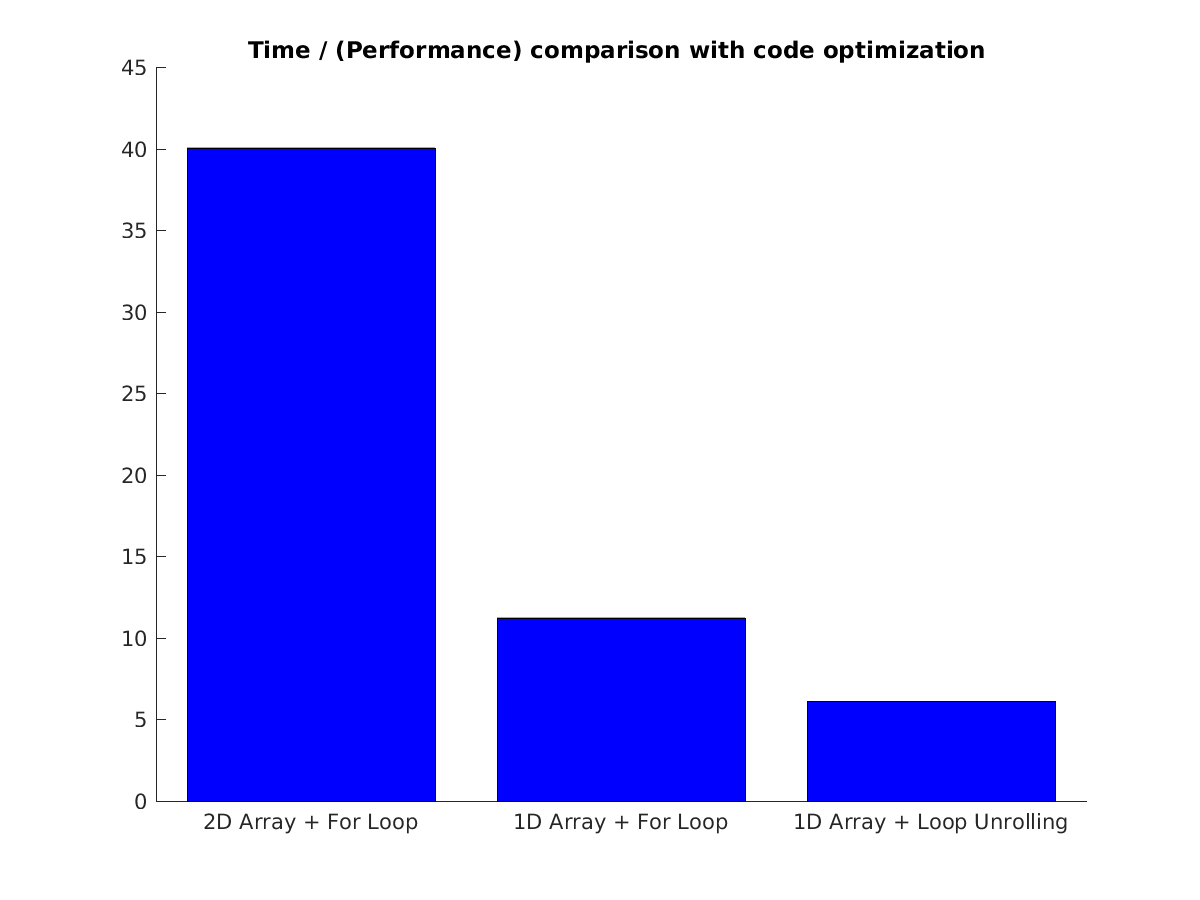
\includegraphics[width = 0.9\linewidth]{code_optimization}
		\caption{Performance improvement for sequential algorithm}
		\label{perimp}
	\end{figure}
	
	\begin{figure}[h]
		\centering
		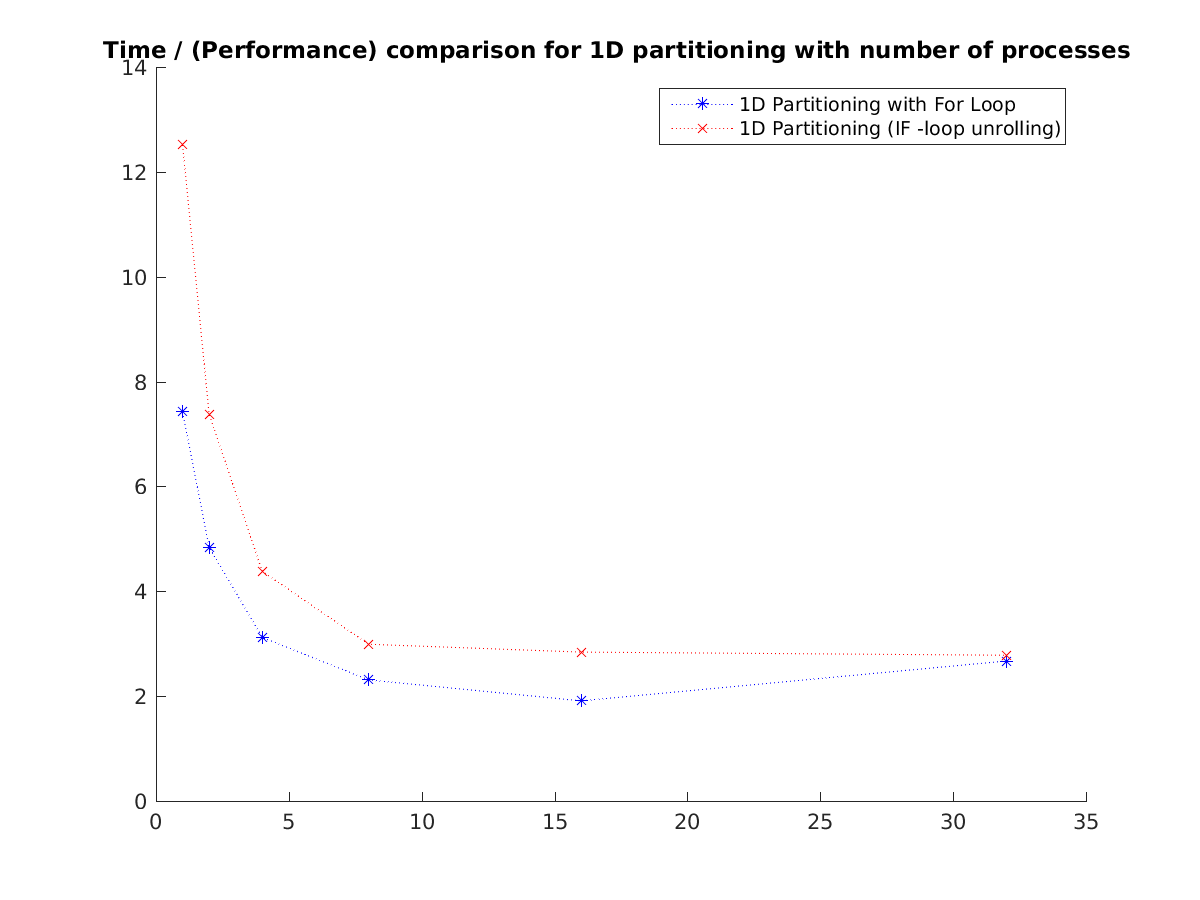
\includegraphics[width = 0.9\linewidth]{1d_optimization}
		\caption{Comparison of improved performance using loop unrolling for 1d parallelized implementation}
		\label{1doptimization}
	\end{figure}
	
	\subsection{Parallel Code - 1D Partition}
	After optimizing the sequential algorithm, further speed up can be achieved by parallelizing the code. It is evident from the problem statement that much of the computations (counting live neighbors) are, more or less, independent of each other. Thus, if this computation is executed simultaneously, we can utilize more computing power of the processor together, to achieve speed-up. Fig.\ref{1doptimization} shows the decline in time for simulating 500 generations of final.data ( 500 $\times$ 500) arena for both - for loop and if else implementations. It is observed that as the partitions become smaller and smaller, the effect of loop rolling diminishes.
	\begin{figure}[h]
		\centering
		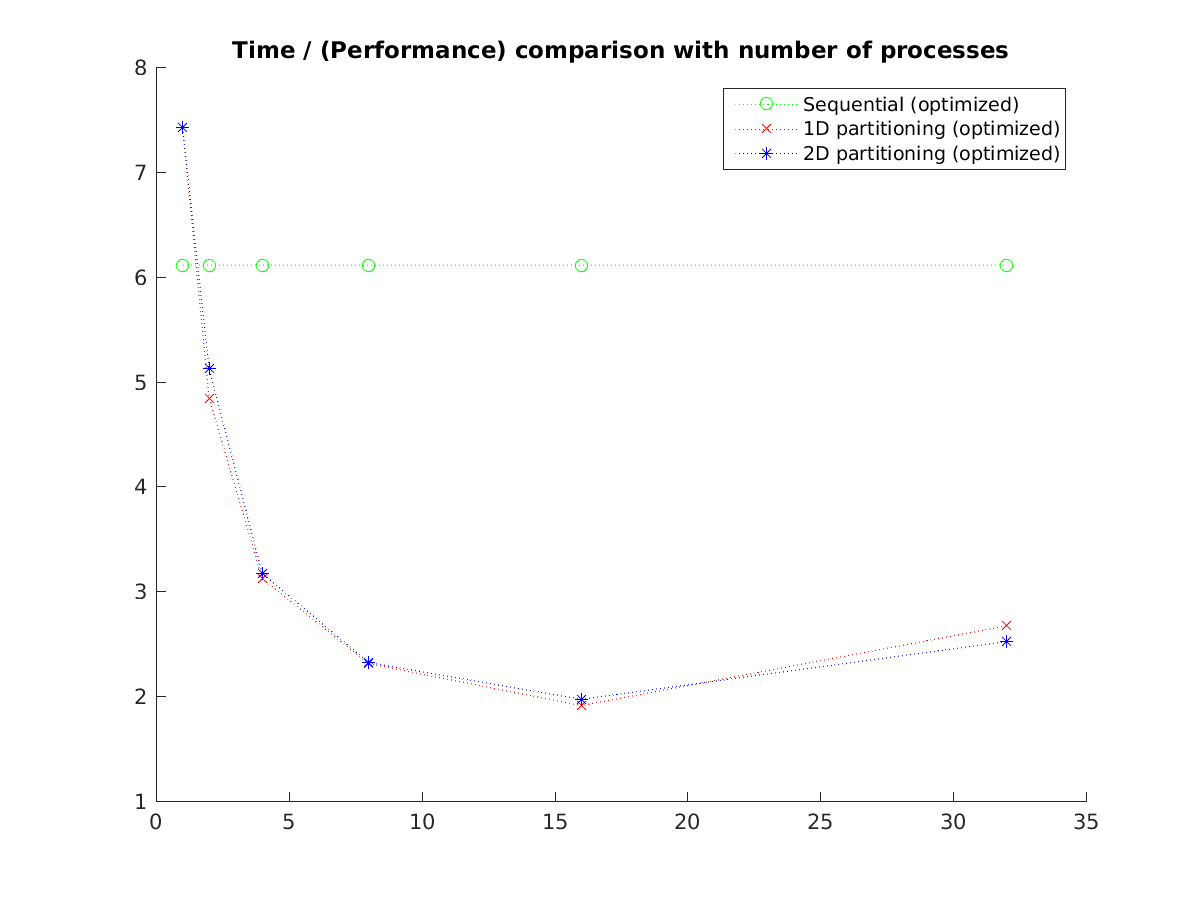
\includegraphics[width = 0.9\linewidth]{all_algo_performance}
		\caption{Performance improvement comparisons for all implementations}
		\label{speedupall}
	\end{figure}
	
	\subsection{Parallel Code - 2D Partition}
	Fig. \ref{speedupall} shows comparison of the speed-up achieved by parallelizing the code for both, 1-D and 2-D partitioning schemes. The performance of both implementations are nearly equal, with 1D being slightly quicker (0.01s) in all cases, probably due to less communication overhead. However, intuitively, this should mean that as the number of partitions increases, the speed-up should diminish for 2D implementation. However, it is found that 1D implementation takes slightly more time than 2D, when number of processes reach 32. This could also be due to system delay.
	\section{Performance Analysis}
	It is shown in Tab. \ref{pa}, that the performance of parallel code is slightly worse than the pure sequential code due to computational overhead of partitioning and communication of data.
	However, there is exponential speed up as we increase the number of processes. Finally, the speedup saturates  after 16 processes, as the time to compute overhead balances the speed up due to parallelization.
	\begin{table}[H]
		\centering
		\caption{No. of Processes vs Time (in secs)}
		\label{pa}
	\begin{tabu} to \linewidth { | X[c] | X[c] | X[c] | X[c] | }
		\hline
		Processes & 1D Partition  & 1D Partition & 2D Partition\\
		 & (For Loop) & (If-Else) & (If-Else)\\
			& Time (in secs) & Time (in secs) & Time (in secs)\\
		\hline
		Sequential  & 11.24 & 6.11 & 6.11\\
		\hline
		 1 & 12.52 & 7.42 & 7.42\\
		\hline
		 2 & 7.38 & 4.84 & 5.12\\
		\hline
		 4 & 4.38 & 3.12 & 3.17\\
		\hline
		 8 & 2.99 & 2.31 & 2.32\\
		\hline
		 16 & 2.84 & 1.91 & 1.97\\
		\hline
		 32 & 2.78& 2.67& 2.52\\
		\hline
	\end{tabu}
	\end{table}
	
\section{Conclusion}
	 Three different implementations where done to simulate Game of Life. 1. Sequential 2. Partitioning data in 1D and communication 3. Partitioning data in 2D and communication. The aim of the project was to understand message passing between processes  using OpenMPI, hence, the optimality of the code was not worked upon - however few improvements are suggested in the report. The speed-up is very drastic as the number of processes are increased but it soon saturates to a constant value - around 2.8 seconds, as the overhead of parallelizing code and communication balances the speed-up achieved. If we further partition the data, there are chances of that the simulation will take more time, as the communication will become the bottle neck.
	 The code for the above mentioned implementations can be found at \href{https://github.com/chiragmajithia/gameoflife}{Github Repository}
	 
\end{document}
 